\documentclass[preprint,aps,pra,floatfix]{revtex4-2}

% preamble.tex — shared packages and macros
\usepackage{graphicx}
\usepackage{amsmath,amssymb}
\usepackage{siunitx}
\usepackage{microtype}
\usepackage{xspace}
\usepackage[usenames,dvipsnames]{xcolor}
\usepackage[colorlinks=true,allcolors=blue]{hyperref}

% Abbreviations
\newcommand{\OSL}{osseous spiral lamina\xspace}
\newcommand{\CPS}{canaliculi perforantes of Schuknecht\xspace}
\newcommand{\ST}{scala tympani\xspace}
\newcommand{\SGN}{spiral ganglion neuron\xspace}
\newcommand{\SGNs}{spiral ganglion neurons\xspace}

% Figures path
\graphicspath{{figures/}}

\begin{document}
\title{Toward Living Cochlear Implants: Using Canaliculi Perforantes to Guide Regeneration}
\author{Akihiro J. Matsuoka}\author{Andrew Carpino}\author{Jae Joon Kim}\author{Audrey Meador}\author{Beatriz Nicolau}\author{Gabriela Fortuno}\author{Hudson Liu}\author{Kiersten Russ}\author{Huimin Zhu}\author{Tifany Nguyen}\author{James Friend}
\affiliation{University of California San Diego; Georgetown University School of Medicine; University of California Los Angeles}
\date{\today}
\begin{abstract}
Cochlear implants (CIs) restore hearing by directly stimulating auditory neurons, yet a persistent electrode--neuron gap constrains spatial selectivity and the fidelity of complex listening. This Topical Review outlines a biohybrid approach that leverages the \CPS\ to guide neurites toward recording/stimulation sites while enabling localized therapy.
\end{abstract}
\maketitle
\
\section*{1. Introduction}

Cochlear implants (CIs) are among the most successful neuroprostheses in clinical use, yet their performance plateaus point to a central limitation of contemporary designs: the millimeter-scale distance between stimulating contacts in the \ST and the excitable elements of the auditory nerve within Rosenthal's canal. Even with perimodiolar arrays, this gap attenuates voltage gradients at the target neurons, blurs spatial selectivity through current spread, and limits the fidelity of temporal and spectral cues that underlie speech-in-noise understanding, music perception, and spatial hearing. In short, we have an engineering interface problem at anatomical scale.

This review advances a biohybrid strategy to address that interface. Rather than relying only on closer metallic electrodes or more aggressive scala insertion, we consider how a device can \emph{cooperate} with living tissue to bridge distance and improve coupling over time. The concept is to integrate guidance and regenerative cues into the implant so that neurites from surviving \SGNs can be \emph{recruited} across natural modiolar pathways toward recording/stimulation sites, while the device simultaneously delivers localized therapies and remains surgically practical.

A key anatomical substrate for such an approach is the network of modiolar microchannels historically described as the \CPS. These small perforations in the \OSL and adjacent modiolar bone are implicated in perilymphatic communication and may provide micro-conduits between the \ST and the neural compartments of the modiolus. If patent in adulthood and accessible from the scala, they could be leveraged for controlled delivery (e.g., neurotrophins, enzymes, RNA cargo, extracellular vesicles) and as permissive corridors for guided neurite extension. The hypothesis we explore here is that pairing these intrinsic pathways with appropriately tuned chemical, mechanical, and electrical cues can reduce effective electrode--neuron distance and increase the number of addressable neural elements without resorting to invasive modiolar drilling.

The notion of a ``living'' or biohybrid implant aligns with broader trends in regenerative bioelectronics, where devices are designed to co-integrate with grafted or host tissue to recover function and enable closed-loop control. Recent perspectives argue that such systems will rely on three classes of cues delivered by the interface: (i) chemical (spatiotemporally controlled release of trophic factors, genes, or vesicles), (ii) mechanical (stiffness, roughness, and topography to bias cell behavior and neurite trajectories), and (iii) electrical (fields and stimulation paradigms to modulate migration, growth, and maturation).\citep{CarnicerLombarte2024AdvMat} The cochlea is a stringent proving ground for these ideas because it demands long-term stability in a compact, fluid-filled, delicate environment, with strong constraints on insertion mechanics, biocompatibility, and serviceability.

We also take advantage of recent progress in accelerating the maturation of human stem-cell–derived neurons, which can shorten preclinical timelines and potentially improve the readiness of transplanted or guided cells. In particular, a four-factor small-molecule regimen (``GENtoniK'')---combining an LSD1 inhibitor, a DOT1L inhibitor, an NMDA receptor agonist, and an L-type calcium-channel agonist---has been shown to rapidly increase neuritogenesis, synaptic puncta, and spontaneous firing across multiple human neuron types and in organoids.\citep{Hergenreder2024NatBiotech} While these data are not yet specific to \SGNs, they showcase a generalizable lever to prime human neurons for integration with engineered interfaces. Importantly, subsequent clarification of synaptic current attribution in that work underscores the need for pharmacological validation when interpreting spontaneous postsynaptic events; we keep this caution in view when proposing readouts and benchmarks.

\textbf{Scope and structure.} Section~2 summarizes the epidemiology and economic burden of hearing loss to motivate the need for higher-fidelity interfaces. Section~3 defines the modiolar microanatomy relevant to electrode--neuron coupling and summarizes routes that matter for delivery. Section~4 reviews regenerative evidence across chemical, mechanical, and electrical modalities, highlighting portable findings and limits. Section~5 surveys interface materials and device architectures that can deliver these cues in the cochlea. Section~6 proposes translational benchmarks and constraints, including surgical feasibility and regulatory considerations for combination products. Section~7 closes with a near-term experimental roadmap and open questions.

By consolidating anatomical clarity with actionable interface strategies, we aim to provide a practical scaffold for researchers developing biohybrid approaches to cochlear implantation, and a shared language for otology, neuroengineering, and materials communities working toward the same goal.

\
\section*{2. Epidemiology and Economic Burden of Hearing Loss}

Hearing loss is a major public health concern that affects everyday communication, education, employment, and healthy aging. In the United States, approximately one in eight individuals (13\%, or about 30 million people) aged 12 years and older has measurable hearing loss in both ears, and 15\% of adults (37.5 million) report at least some trouble hearing.\cite{nidcd2021, cdc2010, cdc2021, wilson2014} These figures meet or exceed the prevalence of other common chronic conditions and emphasize the scale at which hearing impairment consumes health system resources and erodes quality of life.

\subsection*{2.1 Prevalence and risk}
Prevalence rises steeply with age and is compounded by cumulative noise exposure and genetic factors. Globally, disabling hearing loss affects a substantial fraction of older adults, with roughly one quarter of those over 60 years affected, while more than one billion young people are estimated to be at risk of noise-induced, permanent hearing loss.\cite{WHO2025} These epidemiologic trends foreshadow increasing demand for accessible hearing care across the life course.

\subsection*{2.2 Direct and indirect economic costs}
The economic burden of hearing loss spans direct medical spending and substantial indirect costs. Direct costs include clinical evaluations, hearing aids (commonly \$1{,}000--\$4{,}000 per pair), cochlear implantation (\$30{,}000--\$100{,}000 per patient), audiologic rehabilitation, speech--language therapy, and ongoing device maintenance. Indirect costs include reduced productivity and employment: adults with hearing loss have higher odds of unemployment (odds ratio \(\approx 1.98\)), and individual annual income losses up to \$30{,}000 have been reported, aggregating to an estimated \$176 billion per year in the U.S.\cite{SocietyCosts2000, Kim2020, Colburn2019, WHO2025} At the global level, the annual societal cost of unaddressed hearing loss was estimated at \$981 billion in 2020, with quality-of-life losses accounting for about 47\% and a majority of costs (\(\sim\)57\%) incurred outside high-income countries.\cite{McDaid2021}

Strategic investment in hearing care is projected to yield substantial returns. The World Health Organization estimates that scaling essential ear and hearing care interventions to 90\% coverage over the next decade would require an additional \$238.8 billion and generate more than \$2 trillion in productivity gains by 2030.\cite{Tordrup2022} From an individual perspective, early cochlear implantation in children can be cost-saving over the life course: one analysis estimated lifetime healthcare costs of \$489{,}274 for a person born with severe-to-profound loss, reduced to \$390{,}931 (95\% CI \$311{,}976--\$471{,}475) when a cochlear implant is provided before 18 months of age, yielding net lifetime savings of \$98{,}343.\cite{Cejas2024}

\subsection*{2.3 Market context and barriers}
The global cochlear implant market was valued at approximately \$2.42 billion in 2023 and is projected to grow to \$6.63 billion by 2034 (compound annual growth rate \(\sim\)9.0\% for 2024--2034).\cite{globenewswire2025cochlear} Demand is driven by aging populations, persistent noise exposure, and recognition of genetic contributions to hearing loss.\cite{WHO2025} Despite demonstrated benefits, the path to cochlear implantation still presents high barriers: total procedure costs often range from \$50{,}000 to \$100{,}000 when all components of care are included, and access can be constrained by insurance coverage, referral patterns, and center availability. The sector includes established manufacturers such as Cochlear Limited (Australia), Advanced Bionics (Sonova Holding AG, Switzerland), Zhejiang Nurotron Biotechnology Co., Ltd. (China), and MED-EL Medical Electronics (Austria). Regulatory requirements for safety and effectiveness---particularly for novel active implantable devices---and the high cost of research and development contribute to significant barriers to entry, while simultaneously creating opportunities for differentiated, high-value innovation.

\subsection*{2.4 Motivation for higher-fidelity, regenerative interfaces}
Taken together, the epidemiologic scale and the economic burden motivate solutions that improve the benefit-to-cost ratio of hearing care. In the context of cochlear implants, narrowing the effective electrode--neuron distance and increasing the number of addressable neural elements are plausible pathways to improved speech-in-noise understanding, music perception, and spatial hearing. These functional gains would be expected to translate into measurable quality-of-life improvements and economic benefits. This review therefore proceeds from population-level need to the anatomical and engineering questions required to enable ``living'' cochlear implants that cooperate with tissue to improve coupling over time.


\section{\label{sec:AnatRationale}Anatomical Rationale}

%%%%%%%%%%%%%%%%%%%%%%%%%%%%%%
%Figure 1 (Beatriz and Humin)
%%%%%%%%%%%%%%%%%%%%%%%%%%%%%%

\begin{figure}[ht]
  \centering
  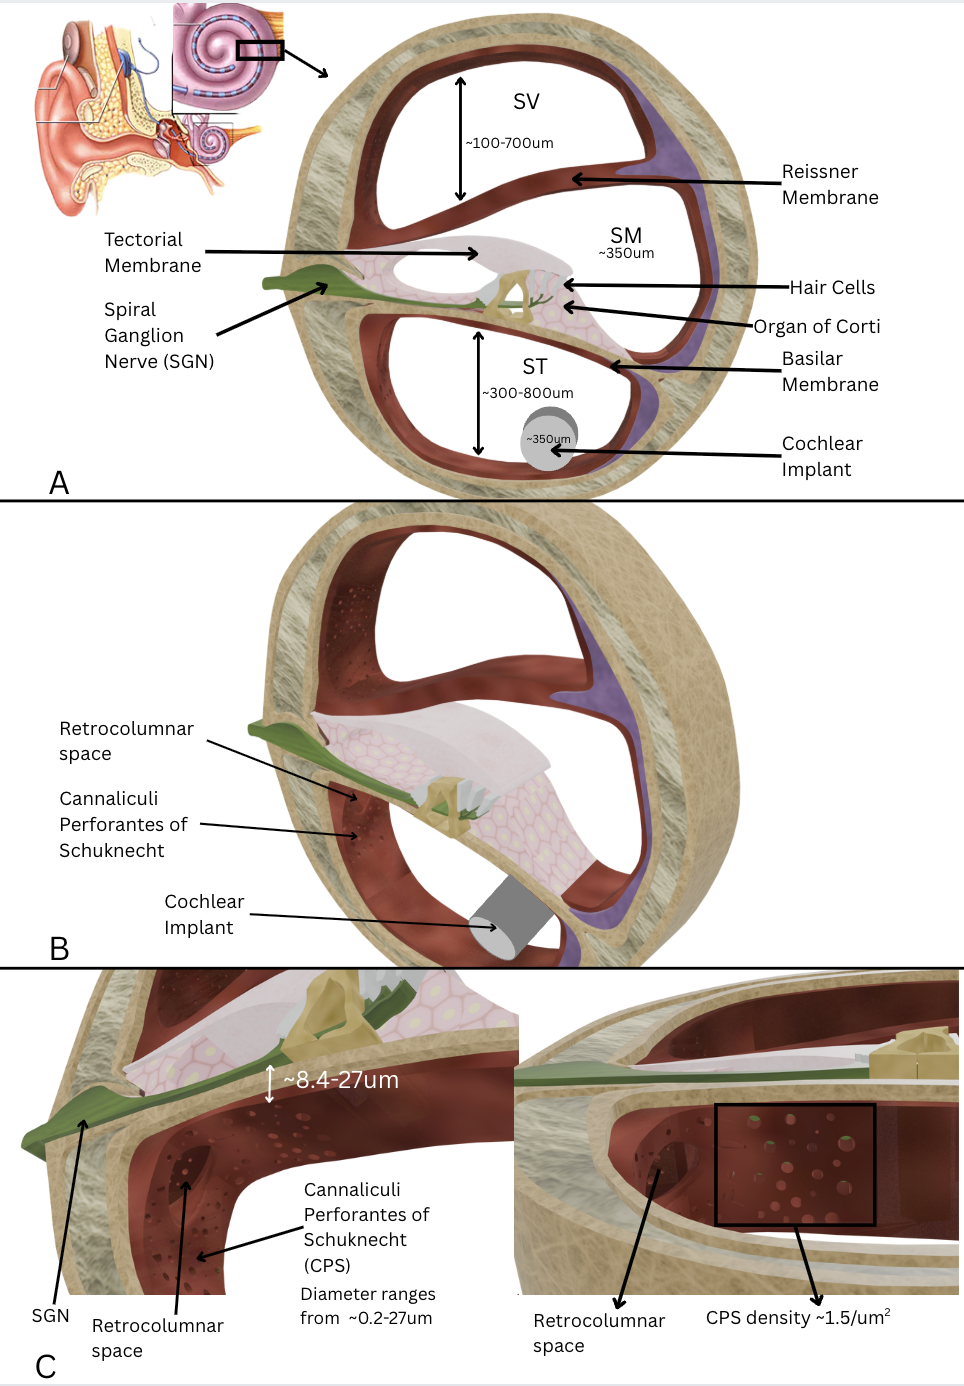
\includegraphics[width=0.8\textwidth]{Figure/3DAnatomyPanel.png}
  \caption{TBW}
  \label{fig:cochlea_overview}
\end{figure}
%%%%%%%%%%%%%%%%%%%%%%%%%%%%%
\subsection{Cochlear scalae in brief}  
The bony labyrinth encloses two perilymph‑filled channels, the \emph{scala vestibuli} and \emph{scala tympani}, which wind around the modiolus and communicate at the helicotrema. Sandwiched between them, the endolymphatic \emph{scala media} houses the organ of Corti on the basilar membrane.  Conventional cochlear implants occupy the scala tympani, placing their contacts within millimeters---but rarely microns---of spiral ganglion neurons (SGNs) embedded in Rosenthal’s canal. Importantly, typical electrode-to-SGN distances are around 0.5–1 mm for modiolus-hugging arrays and up to $\sim1.5-2 mm$ for lateral wall placements \cite{Davis2016}. Even in the best-case scenario, a gap on the order of $10^{2}-10^{3} \mu m$ remains between the electrode and neuron. This physical separation has practical implications: it necessitates current spread through perilymph and bone to reach the neurons, and it underlies why closer electrode positioning (e.g. perimodiolar designs) can reduce stimulation thresholds \cite{Kawano1998}. Furthermore, the distance can vary along the cochlea---apical electrodes often achieve the smallest gaps $\approx0.5 mm$ or less) while mid-cochlear electrodes can be $\approx1 mm$ or more away \cite{Long2014}. These quantitative insights, drawn from human studies, validate that CIs interface with the auditory nerve across a millimeter-scale gulf, rather than forming direct micron-level contact with the neurons. Finally, any natural pores linking the scala tympani to the modiolus are therefore potential highways for drugs, trophic factors, or neurites seeking the electrode array in the scala tympani.


\subsection{Scala Tympani Dimensions and Cochlear Implant feasibility}
\subsubsection{Scala Tympani Anatomy in Humans}
\paragraph{Human[Homo Sapiens]}
:  As briefly mentioned in a previous section, the human scala tympani is a large perilymph-filled canal that narrows from base to apex. Near the basal turn (around the round window region), the ST cross-section is ovoid with a typical vertical height of ~1.2–1.4 mm and width slightly larger \cite{fujiwara2023morphometric}. This corresponds to a cross-sectional area of roughly 2.3 mm² at the base (0°), which then diminishes to about 1.3–1.4 mm² by 180° (half a turn) into the cochlea \cite{fujiwara2023morphometric}. Beyond the basal turn (~360°), the ST lumen becomes more of a flattened triangle in cross-section as it enters the middle and apical turns. The height drops below 1 mm in the upper turns, and the area continues tapering (often $<$ 1 mm² near the apex). Thus, the basal ST can accommodate larger diameters, whereas the apical region is very small and slit-like. Notably, the ST width is consistently greater than its height at any given point \cite{hatsushika1990dimensions}, reflecting the elongated shape of the duct. The human cochlea is ~35–36 mm in uncoiled length (2.5–2.7 turns) and the total ST volume is about 29 $\mu$L \cite{Liu2023FEA}.

\subsection{Canaliculi Perforantes of Schuknecht (CPS)}  
Schuknecht’s original temporal‑bone study (1959) revealed hundreds of microscopic channels piercing the osseous spiral lamina (OSL) from the scala tympani toward the modiolus \cite{schuknecht1959}.  Later histology and scanning‑electron microscopy confirmed that these \textit{canaliculi perforantes} concentrate along the modiolar plate, especially in the basal and middle turns \cite{Schuknecht1963,lim1970,sando1971,masuda1971,tanaka1973}. The CPS are predominantly located on the scala tympani surface of the OSL, in the lower (inferior) bony lamina that underlies the basilar membrane. They are especially numerous in the modiolar (medial) region of the OSL, adjacent to the modiolus where the SGNs are housed \cite{shepherd2004}. Human CPS lumina were measured from 0.2 to 23 $\mu$ m against an OSL thickness that tapers from 26.8 $\mu$ m basally to 8.4 $\mu$ m apically \cite{shepherd2004}.  These dimensions overlap both the caliber of regenerating SGN neurites and the 10--30 $\mu$ m diffusion length of neurotrophins such as NT‑3 or BDNF in perilymph, making each pore a matched conduit for axonal ingress and trophic support.

\subsection{Other modiolar communication routes}  
\begin{enumerate}
\item Trabecular Meshwork: Rask‑Andersen and colleagues identified additional “trabecular meshwork” apertures—up to 100 $\mu$m in the scala vestibuli and 40 $\mu$ m in the scala tympani—plus fenestrations along perivascular and perineural sheaths \cite{raskandersen2006}.  Together with the CPS, they form a porous continuum that contradicts the notion of an impervious modiolar wall, permitting pressure equilibration and macromolecular traffic between perilymph and the SGN somata \cite{raskandersen2006, shepherd2004}.

\item Larger Modiolar Vascular Outlets: In addition, they identified "larger modiolar vascular outlets" as larger openings (up to $\sim$100 $\mu$m) adjacent to the anterior and posterior spiral modiolar veins and arteries, whose function is to permit exchange between perilymph and perivascular spaces, contributing to perilymph homeostasis and potential drug delivery routes. Finally, "mesothelial cell–covered fenestrae" was defined as thin cellular sheets ($<$ 3 $\mu$m) lining the OSL and modiolar surface, interspersed with micropores (up to $\sim$ 40 $\mu$m) on both the scala tympani and scala vestibuli sides. The function of mesothelial cell-covered fenestrae is to provide semi-permeable lining over the bony channels, allowing diffusion of small and large molecules while maintaining fluid compartmentalization \cite{raskandersen2006, shepherd2004}.

\item Mesothelial Cell–Covered Fenestrae: Thin cellular sheets ($<$ 3 $\mu$m) lining the OSL and modiolar surface, interspersed with micropores (up to $\sim$40 $\mu$m) on both the scala tympani and scala vestibuli sides. Mesothelial cell–covered fenestrae allows for exchange between perilymph and perivascular spaces, contributing to perilymph homeostasis and potential drug delivery routes \cite{raskandersen2006, shepherd2004}.

\end{enumerate}

\begin{table}[ht]
\centering
\caption{Quantitative dimensions of perilymph–modiolar passage channels in the basal turn of the human cochlea}
\label{tab:channels_dimensions}
\begin{tabular}{lll}
\toprule
\textbf{Structure / Channel} & \textbf{Dimension (basal turn)} & \textbf{Source} \\
\midrule
Canaliculi Perforantes Schuknecht (CPS) & Mean diameter $5.2 \pm 4.9\ \mu$m (range 0.2--23.0 $\mu$m)       & \cite{ShepherdColreavy2004} \\
Osseous spiral lamina (OSL) thickness & $26.8 \pm 6.0\ \mu$m                                      & \cite{ShepherdColreavy2004} \\
Density of canaliculi (pores/$\mu$m²)   & $1.05 \pm 1.03$ pores/$\mu$m²                                  & \cite{ShepherdColreavy2004} \\
Mesothelial cell–sheet thickness    & $0.3$--$3\ \mu$m                                            & \cite{raskandersen2006} \\
Trabecular‐mesh “fenestrae” size    & Up to $\sim 40\ \mu$m (holes in modiolar wall)             & \cite{raskandersen2006} \\
Modiolar vascular outlets           & Pores up to $\sim 100\ \mu$m                               & \cite{raskandersen2006} \\
\bottomrule
\end{tabular}
\end{table}

\subsection{Functional Pathways and SGN Connectivity Through CPS}
The CPS form a network of microscopic pores through the OSL that directly links the fluid of the scala tympani with the perimodiolar spaces in Rosenthal’s canal \cite{raskandersen2006}. By puncturing the lower plate of the OSL---alongside gaps in its mesothelial lining---and opening into the retrocolumnar trabecular meshwork and perivascular channels of the modiolus, these tiny canals create a continuous perilymphatic pathway from the ST into the SGNs. As a result, the extracellular fluid bathing the SGN cell bodies is essentially the same perilymph that fills the scala tympani, permitting free interchange of ions, nutrients, signaling molecules, and even therapeutic agents or pathogens between these compartments.

Although the true nerve fiber bundles use larger foramina (habenula perforata and modiolar conduits) to enter and exit Rosenthal’s canal, the canaliculi perforantes run alongside and between those fiber routes, serving as perineural and perivascular fluid conduits. Glueckert et al. found nerve fibers in BDNF-treated animals that progressed into CPS. These fibers reveal a myelin layer close to the OSL and within the bony canaliculi but with extreme swelling when entering the scala typani \cite{glueckert2008}. Li et al. also observed SGN neurites projecting across the OSL wall into the ST through the CPS \cite{Li2017}. Similar observations have been reported by others \cite{Staecker1996, Leake2008, Leake2011, Wise2011}.  

\subsection{Distance Between Cochlear Implant Electrodes and Spiral Ganglion Neurons in Rosenthal’s Canal}
Conventional CI electrode arrays reside in the scala tympani and thus are separated from the SGNs in Rosenthal’s canal by the bony modiolus. Multiple anatomical and imaging studies confirm that across patients and electrode positions, the distance between an electrode contact and the SGNs in Rosenthal’s canal generally spans from a few hundred microns up to $\sim$1–2 mm. A detailed CT scan study of perimodiolar arrays reported a total range of $\sim$0.1 mm up to 1.8 mm in electrode-to-modiolus separation \cite{Long2014}. Histological section measurements estimate that in the human basal turn, a lateral-wall electrode may be roughly $\sim$2 mm away from the spiral ganglion (by radial distance). These data support the statement that CI contacts lie within millimeters—but rarely mere microns—of the SGNs\cite{Schmidbauer2023}.

The electrode-to-SGN distance is not uniform along the cochlea; it varies with the cochlear turn and electrode position. Overall, the closest electrode-neuron proximities are achieved in the apical cochlea, with mid-cochlea generally the farthest on average, though patient-specific anatomy causes considerable variability (overall 0.1--1.8 mm range in the cited study) \cite{Long2014}.

\subsection{The Electrode-Neuron Gap Does Matter}
Kawano et al. (1998) performed detailed histopathologic exams of five human cochleae with CIs and measured the distance between each electrode band and the center of Rosenthal’s canal \cite{Kawano1998}. They reported that these electrode-to-SGN distances were in the millimeter range, and importantly found a correlation between greater distance and higher electrical thresholds and comfort levels. In other words, electrodes that sat farther (several millimeters) from the SGNs required more current to evoke hearing, reinforcing that distance is a key factor. The same study noted that intracochlear fibrosis or new bone formation could increase the electrode-modiolus distance, sometimes pushing contacts farther than their design intends. Nadol and colleagues, in histopathologic surveys, likewise estimated distances on the order of 0.5–2 mm and observed that any translocation of an array out of scala tympani (or trauma to the modiolus) can reduce SGN counts, further emphasizing that the electrode-neuron gap matters \cite{nadol1990,Nadol1989}. Computational models and anatomic maps further illustrate these distances. For example, a recent finite-element model by Sriperumbudur et al. (2024) examined electrical stimulation with a perimodiolar CI and assumed a ~0.3 mm gap between the electrode and modiolus as a typical design. This value (300 $\mu$ m) was chosen to reflect a snug perimodiolar placement, yet it still highlights that even in simulation the contacts are not assumed to be touching the neurons (a 0.3 mm gap leaves space for the bony wall and perilymph) \cite{Sriperumbudur2024}. 

\subsection{Surgical implications for biohybrid CIs}  
Because CPS density peaks in the basal OSL, traumatic insertion or aggressive drilling in this region risks sealing the very pathways that a biohybrid implant aims to exploit \cite{shepherd2004}.  Conversely, electrodes engineered with microfluidic ports or neurotrophin‑releasing sleeves could harness these pores to establish steep radial gradients that attract transplanted or residual neurites toward the contacts.  Designing arrays that spare, rather than violate, the CPS therefore becomes as important as thread depth, pitch, or perimodiolar curl.  Leveraging these natural conduits should reduce reliance on bulk diffusion, localize therapy to the modiolus, and ultimately tighten the electrode–neuron interface—a prerequisite for the stem‑cell and material strategies developed in the following sections. Future biohybrid implants are expected to incorporate microfluidic drug delivery (e.g., convection‑enhanced or electrically driven release) to steer regeneration locally within the cochlea \cite{Carnicer-Lombarte:2025aa}.


\section*{4. Regenerative evidence for bridging the gap}\n\n% To be drafted.\n
\section{Surface Modifications to Enhance Neuron--Electrode Interactions}
\label{sec:surface_mods}

A persistent barrier to cochlear implant (CI) performance is the micrometer–millimeter gap between the electrode surface and spiral ganglion neurons (SGNs), which forces large current spread and degrades channel selectivity. In a biohybrid CI, surface engineering can be used to (i) lower the electrochemical barrier at the interface, (ii) physically guide neurites toward the contacts, and (iii) suppress the early protein fouling and chronic inflammatory cascades that otherwise raise impedance and reduce neural proximity. Below we outline four complementary approaches and design considerations for integrating them into a unified, regeneration‑supportive interface.

\subsection{Approach 1: Microstructured Electrode Surfaces}
Microscale topography can bias SGN neurite alignment and extend the effective “capture radius” of the contact. Repeating ridge–groove patterns (periods $\sim$5–20\,\textmu m; depths $\sim$1–5\,\textmu m) consistently increase neurite alignment along the pattern axis and improve turning fidelity at corners, effects attributed to growth‑cone mechanosensation and downstream calcium signaling \cite{Wang2013,Chen2014}. In vivo, microgrooved CI electrodes show the expected trade‑off: improved neurite guidance and interface stability must be balanced against insertion trauma if protruding features are too tall or sharp \cite{Lee2019}. Practical guidance is to keep features shallow and rounded, blend them into a compliant coating (below), and co‑present permissive ECM ligands where appropriate (e.g., laminin stripes) to amplify topographic bias without adding stiffness discontinuities at the leading edge \cite{Evans2007LamininFibronectin,Vega1995LamininCollagenIV}.

\subsection{Approach 2: Conductive and Electroactive Coatings}
Roughened noble metals and electroactive polymers reduce interfacial impedance and increase charge‑injection capacity. PEDOT and polypyrrole (PPy) films, including interpenetrating PEDOT–hydrogel networks, produce large, stable impedance reductions and better charge transfer under chronic stimulation \cite{Venkatraman2011-ql,Goding2017,Dalrymple2020,ABIDIAN20081273}. Biofunctionalization of these films (e.g., RGD‑ or peptide‑modified PEDOT; drug‑loaded PPy) further supports cell adhesion and controlled factor release directly from the electrode surface \cite{Chikar2012}. For a biohybrid stack, a thin PEDOT (stability) over PPy (loading) can sit beneath a soft, conductive hydrogel to match tissue modulus while preserving low impedance and space for embedded trophic depots (Section~\ref{sec:materials_stack}, if used). Key checks are adhesion under accelerated aging, charge density limits in saline that mimic perilymph, and retention of low noise after sterilization \cite{Venkatraman2011-ql,Dalrymple2020}.

\subsection{Approach 3: Antimicrobial and Pro‑healing Interfaces}
Early bacterial colonization and the ensuing foreign‑body response are major risks for any chronic implant. Polydopamine (PDA) is a versatile primer that improves coating adhesion and can present bioactive peptides; on silicone CI carriers, PDA–peptide films increase cell adhesion and viability \cite{Schendzielorz2017}. Zwitterionic chemistries (e.g., sulfobetaines) grafted or deposited onto CI materials markedly reduce nonspecific protein adsorption and leukocyte adhesion, lowering inflammation in vivo and improving stability at the electrode–tissue interface \cite{Horne2023,Chen2023-ba}. Complementary strategies include antioxidant/antibiofilm polysiloxane coatings (e.g., N‑acetyl‑L‑cysteine–modified siloxanes) that inhibit biofilm formation while maintaining polymer stability under physiological conditions \cite{Cozma2021-jb}. In a layered design, these chemistries can be placed as the outermost surface (tissue‑facing) while leaving the underlying electroactive layers to handle charge transfer.

\subsection{Approach 4: Anti‑fouling and Anti‑biofilm Surface Chemistry}
Hydration‑rich, charge‑balanced surfaces (zwitterions; highly hydrophilic brushes) resist the protein conditioning film that otherwise seeds fibroblast/macrophage recruitment and biofilm growth. Recent zwitterion‑modified CI materials showed large reductions in postoperative infection and inflammatory cell adhesion, with preservation of low impedances relative to unmodified controls \cite{Chen2023-ba,Horne2023}. When antimicrobial action is required (e.g., revision or high‑risk cases), chemistries that provide sustained bactericidal activity without cytotoxicity to SGNs are preferred; NAC‑functional polysiloxanes are one such route compatible with elastomeric carriers \cite{Cozma2021-jb}. These layers should be validated for (i) stability under electrical pulsing, (ii) sterilization compatibility, and (iii) retention of anti‑fouling function after mechanical insertion testing.

\paragraph{Design guidance (summary).}
\begin{itemize}
	\item \textbf{Start with impedance and modulus:} pair a stable electroactive coating (PEDOT $\pm$ PPy) with a compliant conductive hydrogel to lower $Z$ and match cochlear tissue stiffness \cite{Venkatraman2011-ql,Goding2017,Dalrymple2020}.
	\item \textbf{Add gentle topography for guidance:} shallow ($\lesssim$2--3\,\textmu m) ridges/grooves aligned to the longitudinal axis can bias neurite extension without adding insertion risk \cite{Wang2013,Chen2014,Lee2019}.
	\item \textbf{Cap with anti‑fouling chemistry:} use zwitterionic or PDA‑primed, zwitterion‑grafted layers as the tissue‑facing surface; add targeted antimicrobial/antioxidant functionality if clinically indicated \cite{Horne2023,Chen2023-ba,Cozma2021-jb,Schendzielorz2017}.
	\item \textbf{Co‑design with biochemical release:} where trophic support is provided (e.g., BDNF depots described earlier), align microtopography with release gradients to steer neurites toward contacts while maintaining low impedance \cite{Chikar2012,Goding2017}.
\end{itemize}
Taken together, these surface modifications provide a practical path to shrink the functional electrode–neuron gap and stabilize the interface over time—both prerequisites for any biohybrid CI that aims to recover finer spectral resolution.

\section*{6. Translational benchmarks and constraints}\n\n% To be drafted.\n
\section*{7. Roadmap and open questions}\n\n% To be drafted.\n
\bibliography{bib}
\end{document}
